\newpage
\section{Ejercicio 7}
	\subsection{Analisis del Schedler}

	Para entender el schedler, hemos corrido  una serie de tareas .

	\begin{figure}[ht]
		\begin{center}
			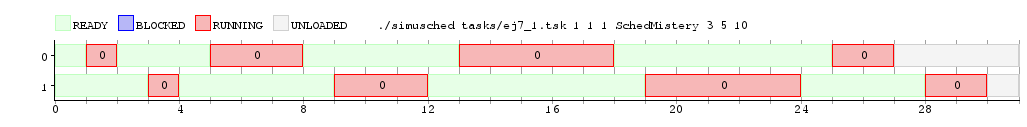
\includegraphics[width=1\columnwidth]{imagenes/ej7_1.png}
			\caption{Dos \texttt{TaskCPU} con 20 quantums.}
		\end{center}
	\end{figure}

	Se puede apreciar que cuando una  tarea acaba sus quantums, es quitada de la cola donde esta y es  agregada en la siguiente cola con menor prioridad , si es posible , en caso contrario quedara en la cola donde pertenece (La de menor prioridad) . Una vez que el schedler desencola todas las tareas pendientes en una cola pasa a la siguiente.


	\begin{figure}[ht]
		\begin{center}
			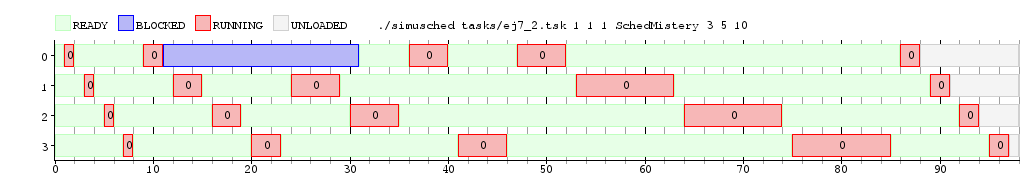
\includegraphics[width=1\columnwidth]{imagenes/ej7_2.png}
			\caption{Un \texttt{TaskCPU} corriendo con 20 quantums y tres \texttt{TaskAlterno} alterando 2 quantums de uso de kernel , 1 de bloqueo}
		\end{center}
	\end{figure}

	Como se puede apreciar este schedler permite starvation, es que las tareas con pocos ó ningun bloqueo se acumulen en las colas con menor prioridad, esperando ha que las tareas de mayor prioridad terminen para que les toque a ellas.
	Cuando una tarea se desbloquea , es la proxima tarea ha correr y su nivel de prioridad aumenta en uno.

	\begin{figure}[ht]
		\begin{center}
			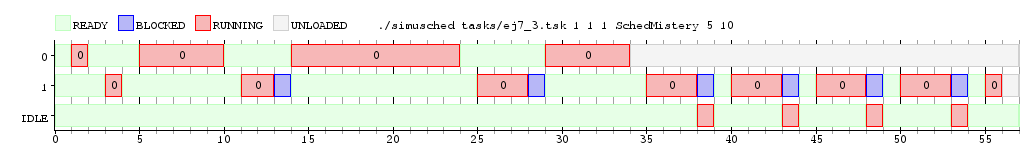
\includegraphics[width=1\columnwidth]{imagenes/ej7_3.png}
			\caption{Un \texttt{TaskCPU} corriendo con 20 quantums y un \texttt{TaskAlterno} alterando 2 quantums de uso de kernel , 1 de bloqueo al principio y despues 4 y 2.}
		\end{center}
	\end{figure}

	Como se ve la tarea IDEL  actua como se espera , cuando no hay nada para correr , corre la IDEL.

	Los quantums asignados a las colas de prioridad son 1 quatum a la de maxima prioridad y los argumentos pasados por parametro son las siguientes prioridades.

	\subsection{Implementación del Schedler}



